\subsection{MOSFET and Driver}
A MOSFET (Metal-Oxide-Semiconductor Field-Effect-Transistor) is used to control the amount of power which is delivered to the Load. The MOSFET must be able to handle a big amount of current produced by the Generator (\SI{44}{\ampere}).

The chosen transistor is a IRFP260N power MOSFET. This is an N-type MOSFET and is rated to be able to handle a drain-current I\textsubscript{D} of \SI{50}{\ampere} and a drain-source-voltage V\textsubscript{DSS} of \SI{200}{\volt}. Furthermore it is specified to have a very low on-resistance of \SI{40}{\milli \ohm} and can operate up to a temperature of \SI{175}{\celsius}.

A MOSFET-driver is needed in order to fully control the MOSFET's gate. The driver is needed to amplify the input-signal as:
\begin{itemize}
	\item The MOSFET's gate has a capacitive reactance which means that the gate must be charged before the MOSFET can conduct current. The charging-process would be extremely slow if it was done by the PSoC and the gate-current must be amplified in order to speed up the process.
	\item The MOSFET operates with a gate-source-voltage of \SI{12}{\volt}. This cannot be supplied by the PSoC and the gate-voltage must be amplified. 
\end{itemize}

In order to calculate the amount of current which is needed to charge the gate, the specified values for the Total Gate Charge Q\textsubscript{g} and the rise-time t\textsubscript{r} are found in the MOSFET's datasheet. These values are specified as:
\begin{equation}
\begin{split}
	Q_g &= \SI{234}{\nano \coulomb}\\
	t_r &= \SI{60}{\nano \second}
\end{split}
\end{equation}
Assuming a constant value the required gate-current can then be calculated as:
\begin{equation}
	I_{gate} = \frac{Q_g}{t_r} = \frac{\SI{234}{\nano \coulomb}}{\SI{60}{\nano \second}} = \SI{3.9}{\ampere}
\end{equation}
The chosen driver is a MCP1407 High Speed Power Driver. This driver is specified to be able to handle a large output-current of \SI{6}{\ampere} and can supply the MOSFET with \SI{12}{\volt}. It shold also be able to charge and discharge the MOSFET's gate in about \SI{40}{\nano \second}.

\begin{figure}[H]
	\centering
	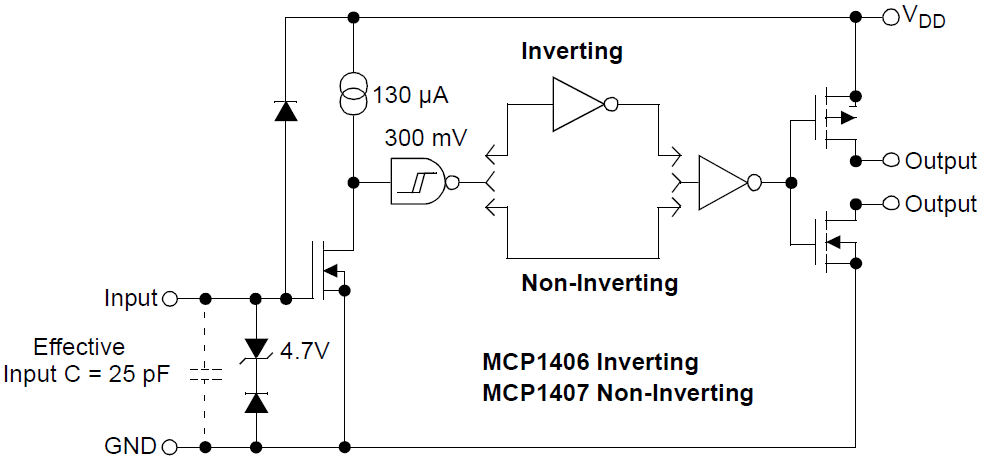
\includegraphics[width=0.7\linewidth]{Hardware/LoadSystem/GateDriver}
	\caption{MCP1407 High Speed Power Driver internal circuit}
	\label{fig:MOSFETDriverInternal}
\end{figure}

The MOSFET-driver is configured such that the outputs are connected with the MOSFET's gate through a \SI{3.3}{\ohm} resistor and the input is connected with the PSoC's output. The driver's positive supply line V\textsubscript{CC} is connected with the 12 VDC line in parallel with a \SI{1}{\micro \farad} and a \SI{0.1}{\micro \farad} capacitor. The driver's remaining pins are connected to ground as specified in the datasheet. The implemented design is seen below.

\begin{figure}[H]
	\centering
	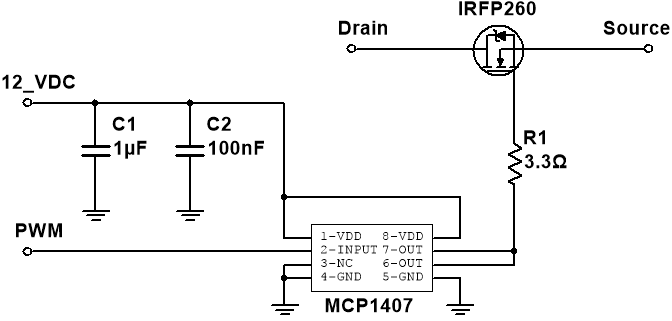
\includegraphics[width=0.7\linewidth]{Hardware/LoadSystem/MOSFET}
	\caption{Configuration of MOSFET and driver in the system}
	\label{fig:MOSFETCircuit}
\end{figure}